%==========================================================================
%HTTP/2
%2015/04/08 (rumeda@mikilab.doshisha.ac.jp)
%==========================================================================

\documentclass[a4j,9pt,twocolumn]{jsarticle}
\usepackage{mlm2.0}
\usepackage{epsf}
\pagestyle{plain}


\begin{document}
\twocolumn[
%---------------------------------------------------------------------------
% ヘッダ    書式:\beginheader{回}{年}{月}
%---------------------------------------------------------------------------
\beginheader{161}{2015}{4}


%---------------------------------------------------------------------------
% 発表題目    書式:\title{日本語}{英語} 「\\」で改行できます
%---------------------------------------------------------------------------
\title%
{HTTP/2}%


%---------------------------------------------------------------------------
% 著者名      書式:\author{日本語著者名}{英語著者名}
%---------------------------------------------------------------------------
\author{梅田 玲旺,松井 健人,内村 祐之,市川 燿\\Reo UMEDA,Kento MATSUI,Yushi UCHIMURA,Hikaru ICHIKAWA}

%---------------------------------------------------------------------------


\endheader

%\begin{abstract}
%---------------------------------------------------------------------------
%Recently, a DVD attracts attention along with the image and the digitization of the sound. The standards of these DVD are complicated. So, in this paper, the standards of the DVD are summarized and the DVD of the next generation is refered. 
%---------------------------------------------------------------------------
%\end{abstract}
\vspace{3mm}
]




%---------------------------------------------------------------------------
% 本文
%---------------------------------------------------------------------------

\section{はじめに}
今ではもうインターネットをたくさんの人々が閲覧することは普通の光景となった.
近年はスマートフォンを使いインターネットを観覧する人が非常に多くなった.
\\ 1人一台でインターネットにいつでもどこででもできるようになりインターネット全体の通信量は非常に増えてきた.
\\ 最近のWebサイトではサーバとブラウザ間でやり取りをしなければならないデータの量が増えてきている.
\\ そのためページを表示するのに遅くなる要因になる。なので通信を効率よくして通信量を減らす必要がある.

\section{HTTP}
HTTPはHypertext Transfer Protocolの略称であり
サーバとブラウザ間でテキストをを主にやり取りするために開発された通信の約束である.
\\ 1990年ごろ物理学者のティム・バーナーズ・リー氏が
組織内という範囲の限られた情報にアクセスするために設計をした.
\\ HTTP/0.9はテキストがメインの簡単なやり取りのみだった.
\\ その後1996年にHTTP/1.0の仕様が公開され音楽や画像,動画などの様々なデータのやり取りに対応した.
\\ 1999年に公開されたHTTP/1.1は複数のデータを効率よく転送するため
通信路を通信するたびに確保するのではなく通信路を繋いだままにする仕様になっていた.
\\ しかし,通信のメッセージはテキスト形式でデータが大きい.
また大きい要求があるときは複数要求を送っても応答が来るまで時間がかかるなど問題もある.


\section{HTTP/2}
\subsection{HTTP/2の特徴}
HTTP/2では通信の効率化を目的として,以下の要素から成り立っている.

\begin{itemize}
 \item  通信のメッセージがテキスト形式から形の決まったバイナリ形式
 \item 通信路の効率化
 \item HTTPヘッダの圧縮
 \item サーバから必要なデータの付与
\end{itemize}

よってHTTP/1.1とHTTP/2の違いは以下のTable\ref{table00}である.

\begin{table}[h]
\begin{tabular}{|c|l|l|l|}
\hline
  & HTTP/1.1 & HTTP/2  \\ \hline
サーバとの &  複数& 1\\
接続数&&\\ \hline
サーバから & ブラウザの & ブラウザの送信順番\\
返信の順番&送信順番通り&に関係しない \\ \hline
メッセージの & テキスト形式 & バイナリ形式\\
表現&&\\ \hline
ヘッダ圧縮 & なし & あり  \\ \hline
サーバから & なし & あり  \\
必要なデータ&&\\
付与&&\\ \hline


\end{tabular}
\caption{HTTP/1.1とHTTP/2の違い}
\label{table00}
\end{table}


\subsection{ストリーム}
HTTP/2でのやり取りをするためには相手までの通信路を確保し「ストリーム」という
仮想通信路を作る.
\\ ストリームは通信路の中にさらに小さな通信路があるかのようにしていている.
それぞれにはナンバーが割り振られ「ストリームID」と呼ばれる.
\\ そして,HTTP/2では複数のストリームを使うことで
サーバとのやり取りを同時に複数している.イメージをFig.\ref{figHTTP200}に示す.

\begin{figure}[h]
\centering
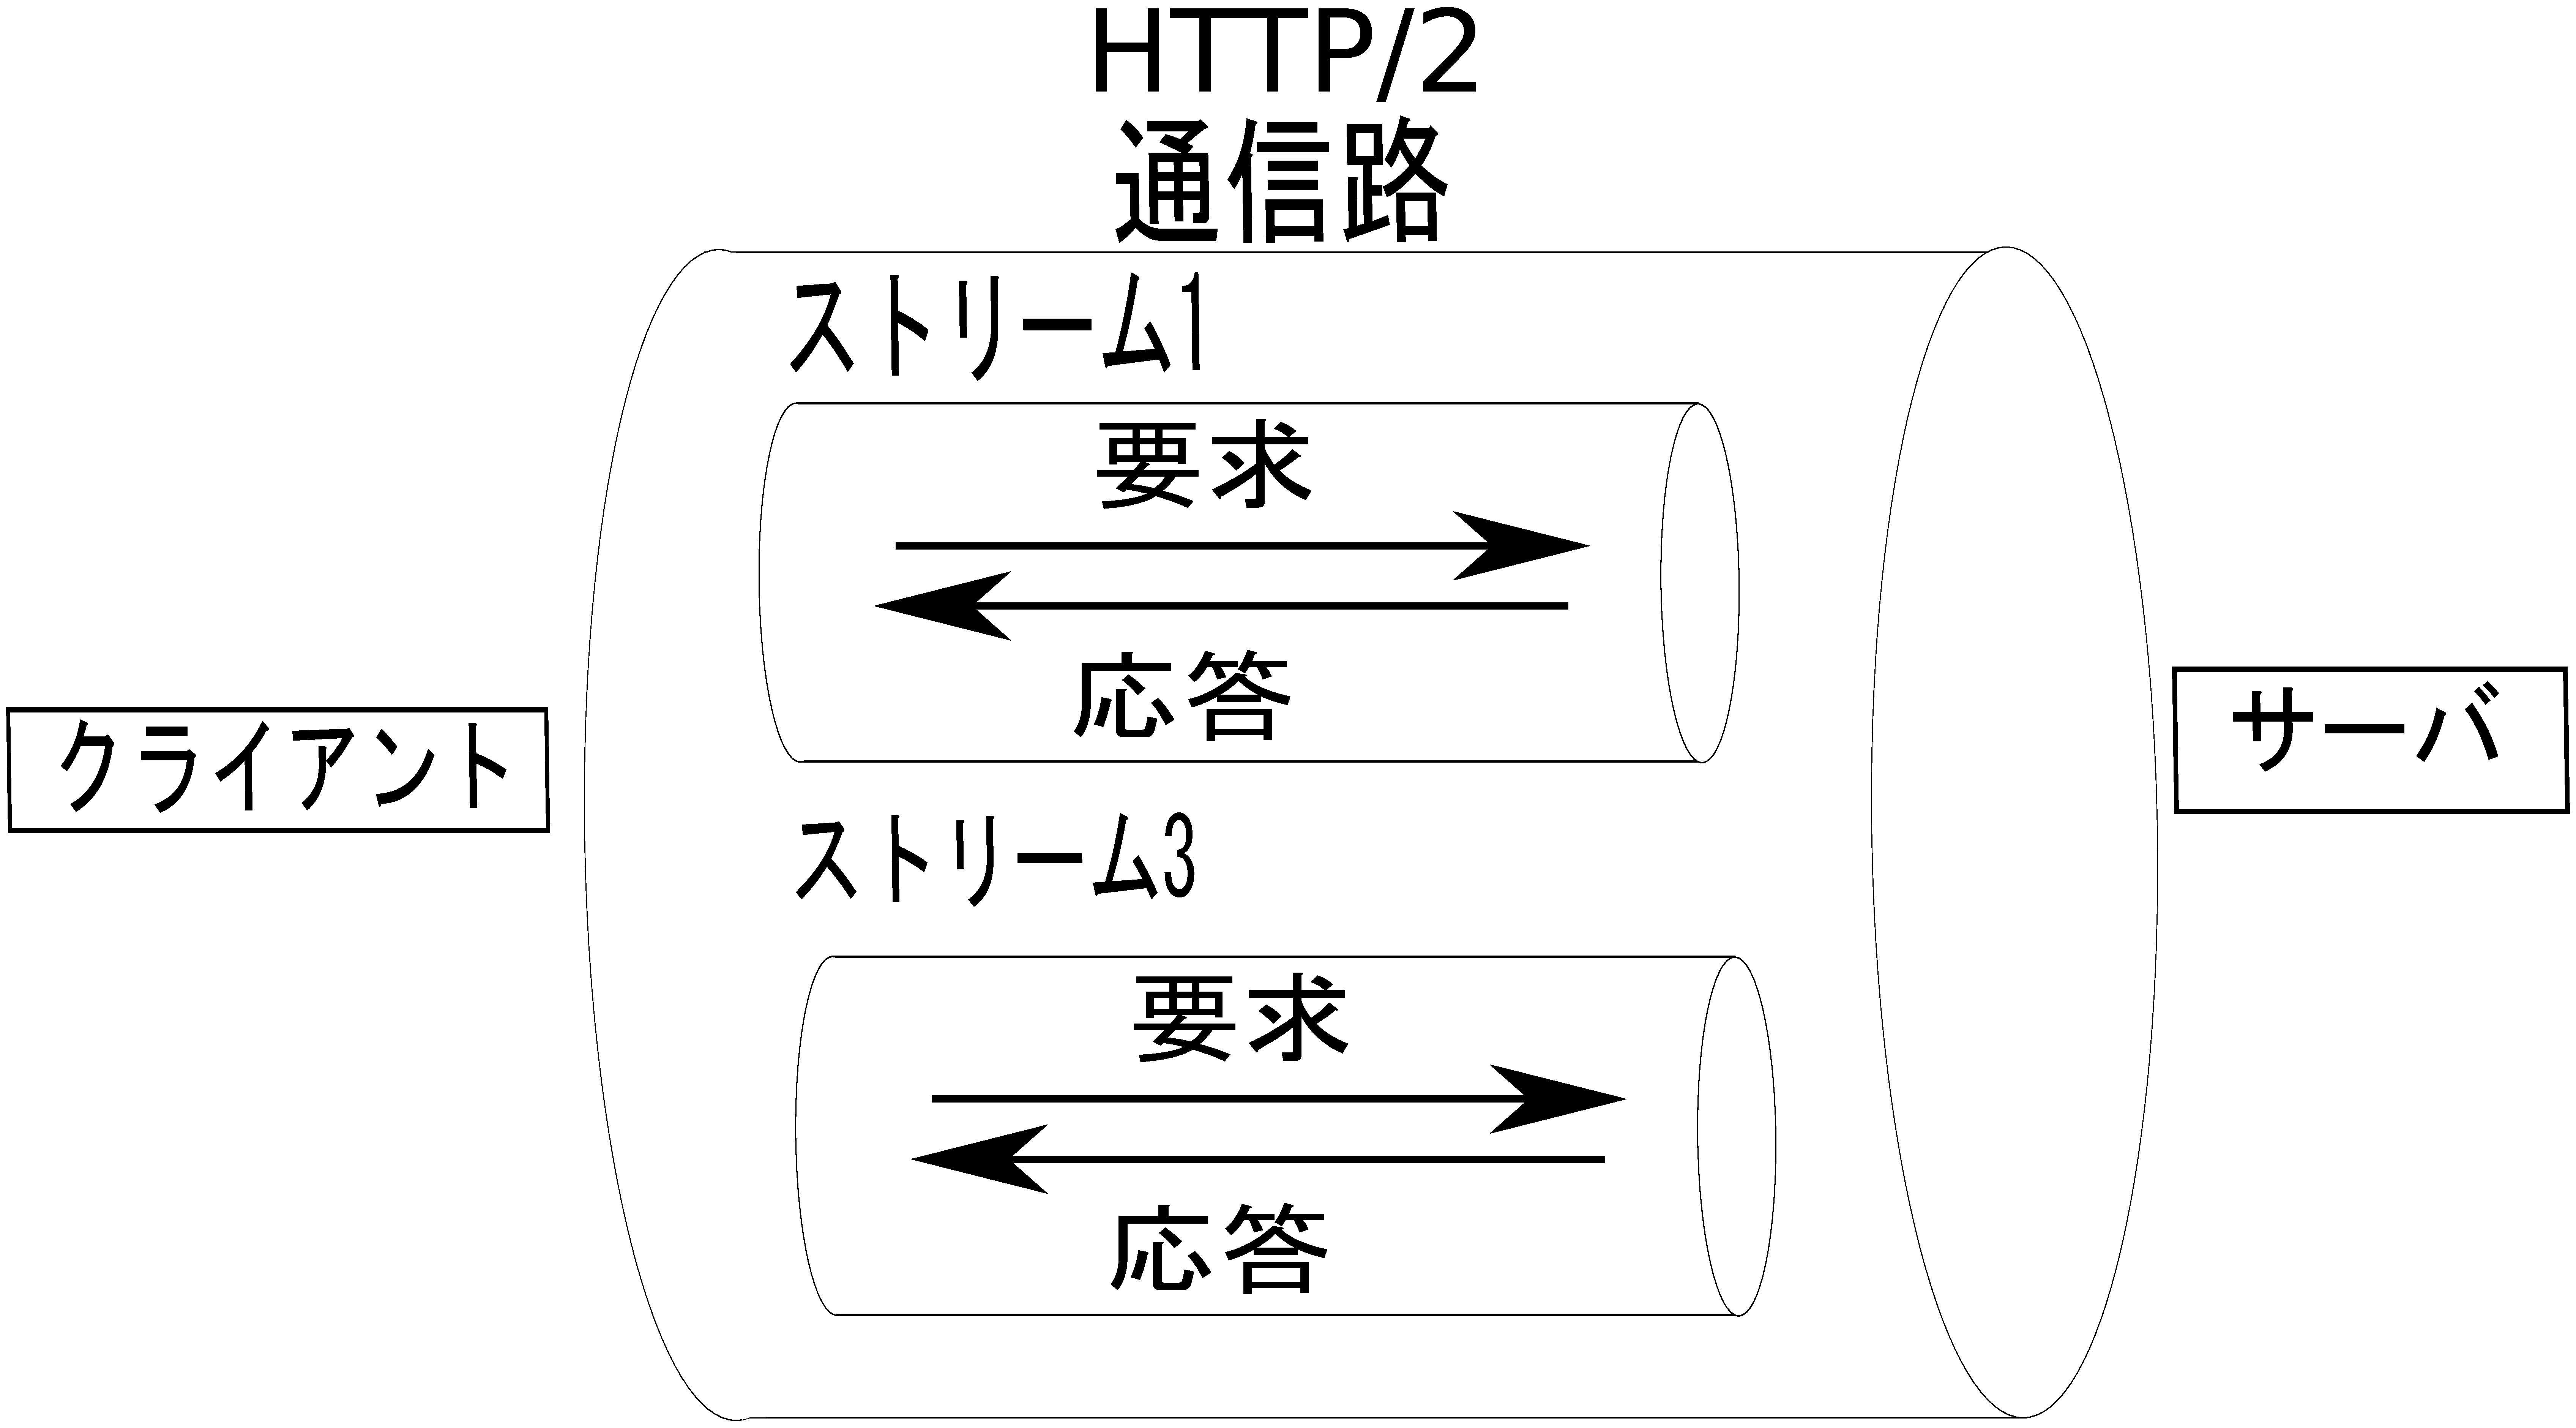
\includegraphics[width=80mm]{img/TCPco6.eps}
\caption{HTTP/2の通信路}
\label{figHTTP200}
\end{figure}

同じことをするときHTTP/2では1つの通信路しか使っていないが
HTTP/1.1では複数の通信路を使っている.イメージをFig.\ref{figHTTP1.1}に示す.


\begin{figure}[h]
\centering
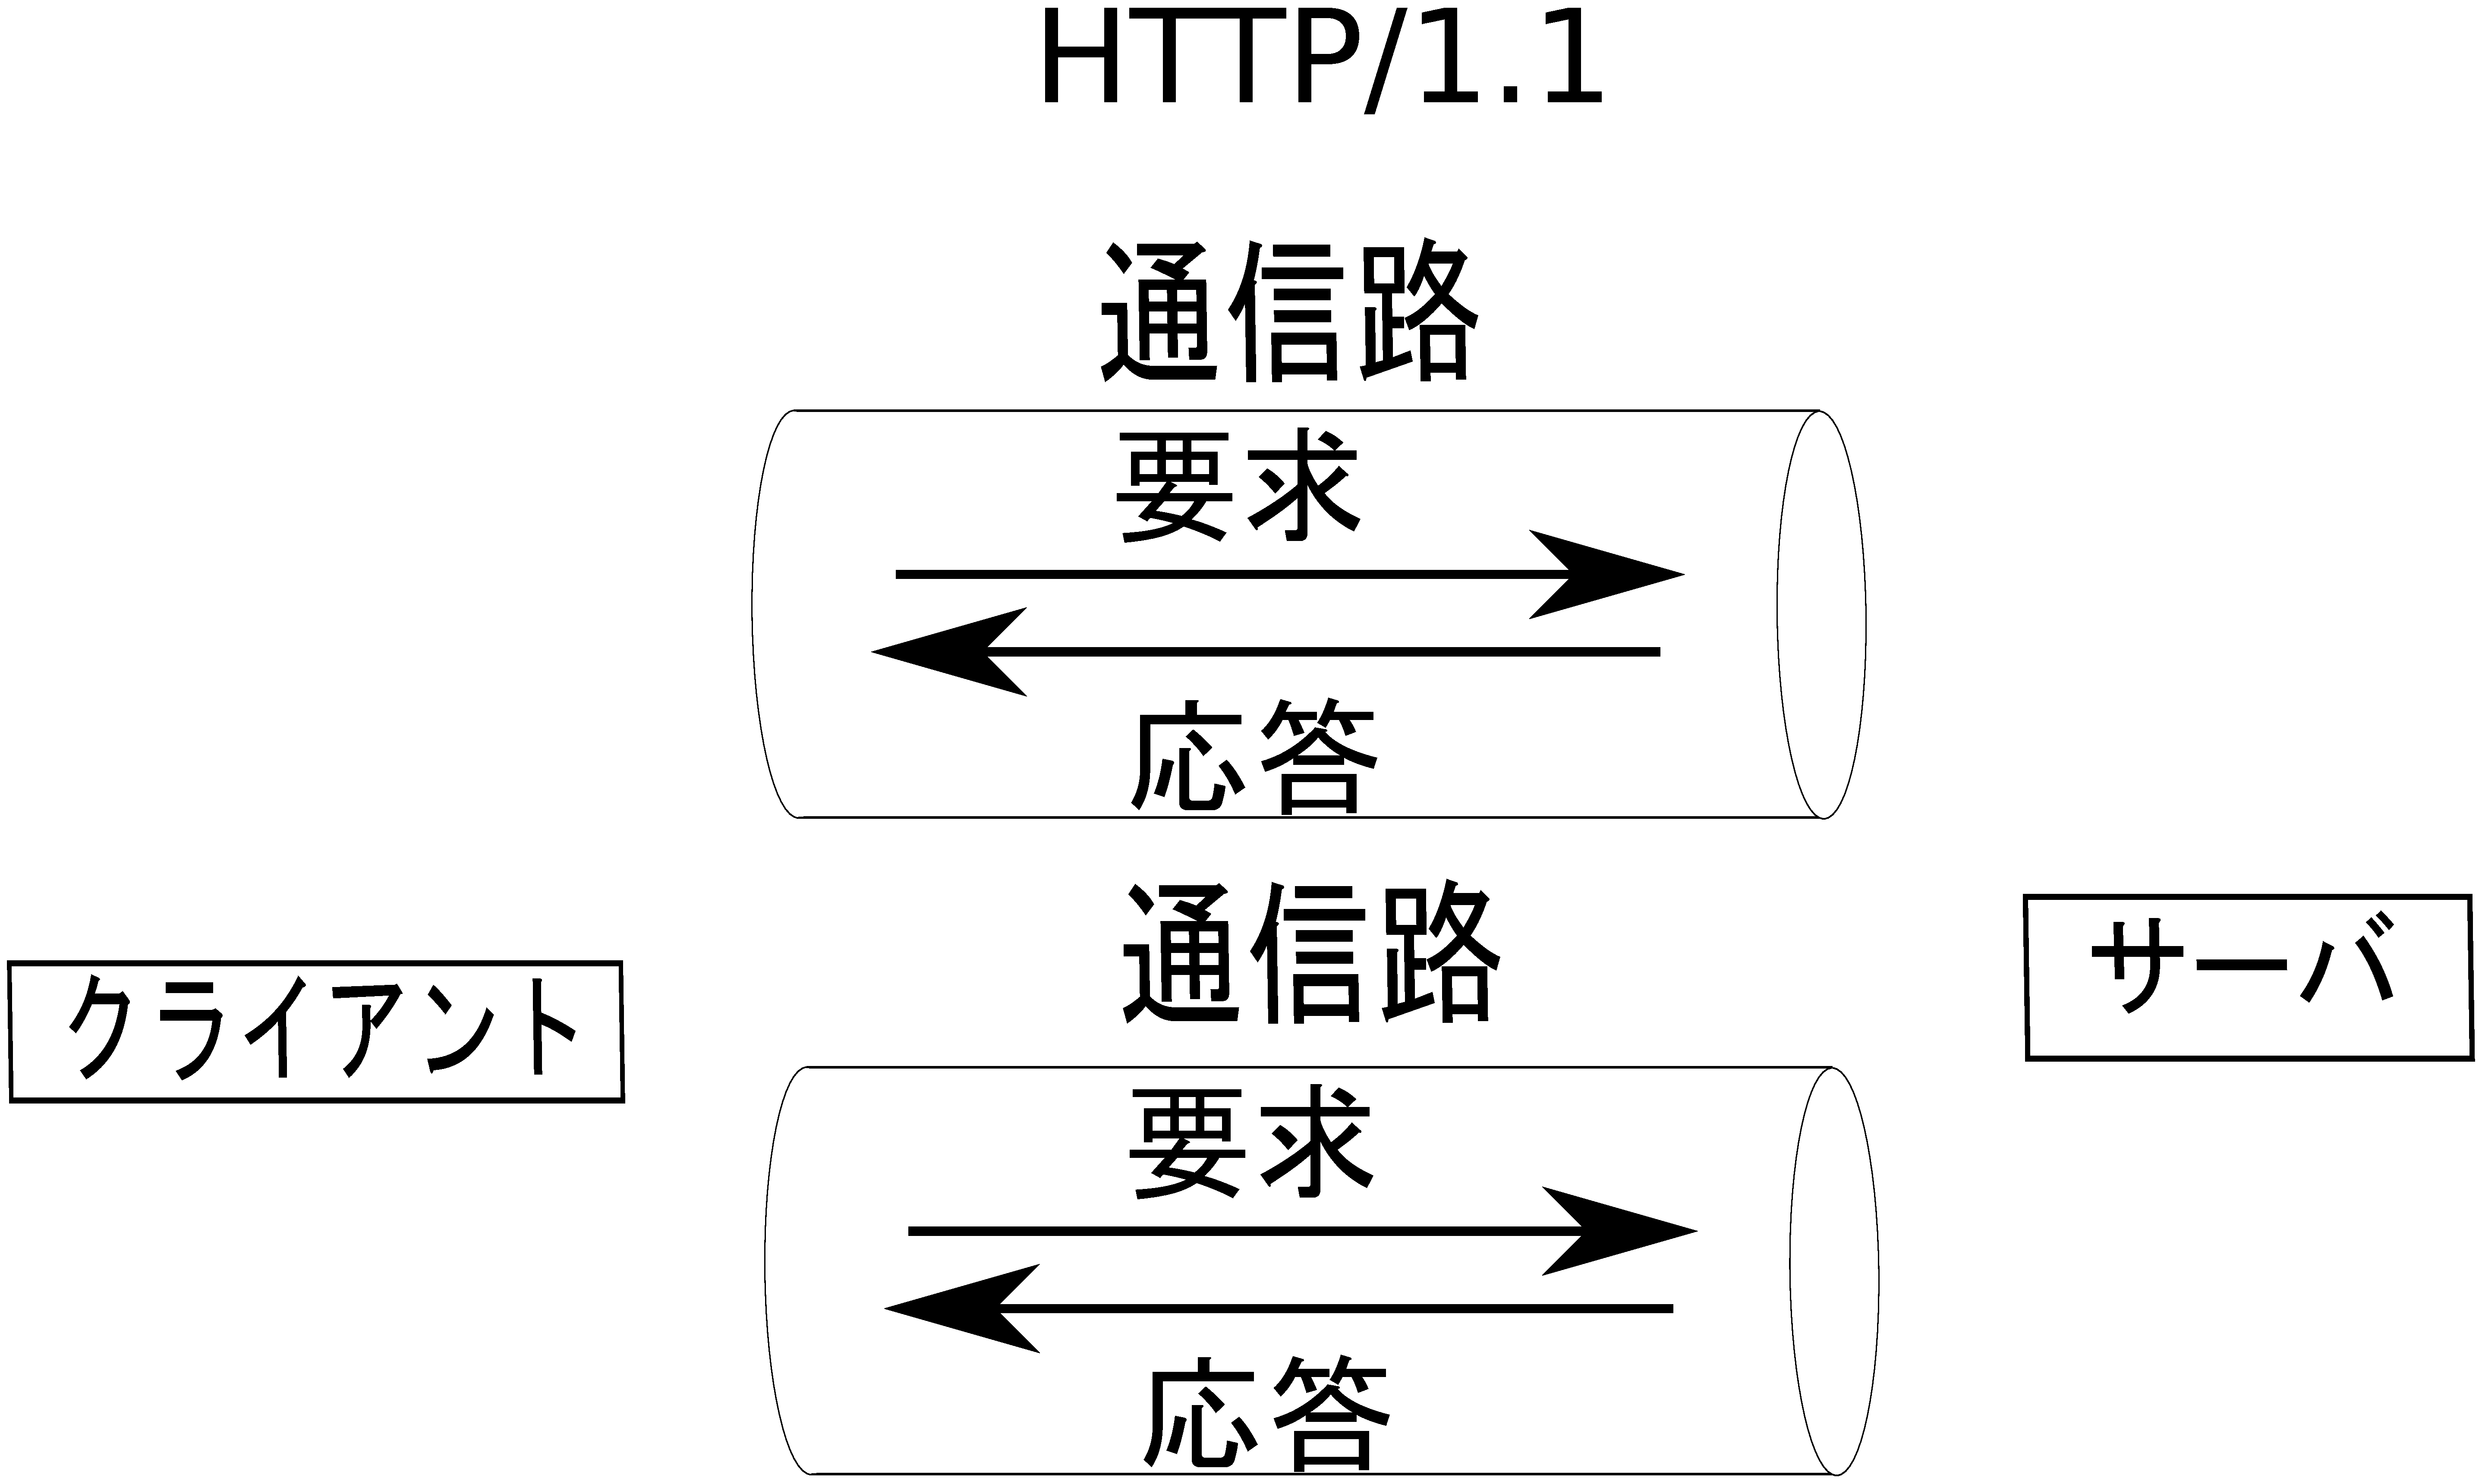
\includegraphics[width=80mm]{img/TCPco5.eps}
\caption{HTTP/1.1の通信路}
\label{figHTTP1.1}
\end{figure}

このため,HTTP/2はネットワークに対して負担が少なくなる.
ブラウザから複数の要求を送ったとき応答がHTTP/1.1とHTTP/2では異なる.
イメージをFig.\ref{HTTPrespons}に示す.


\begin{figure}[h]
\centering
\includegraphics[width=80mm]{img/RR3.eps}
\caption{HTTPの要求と応答}
\label{HTTPrespons}
\end{figure}

HTTP/1.1では要求の順にしか応答は返せない.
しかしHTTP/2では順番に関係なく返すことが出来る.
\\ よってHTTP/2では処理の速いものから応答を返すことができるようになり
全ての応答が帰ってくる時間が速くなる.
\\ また,HTTP/2ではブラウザ側がストリームに「優先度」をつけることが出来る.
そうすると速く帰ってきて欲しい要求のほうが速く応答が帰ってくるようになる.
\\ 例えば文字の要求を先に送り,後から優先度の高い画像の要求を送ると
画像の応答が速く帰ってくる.



\subsection{バイナリの使用}
HTTP/2になると通信のメッセージを「フレーム」という決まった形でやり取りをしている.
\\ フレームは以下Fig.\ref{HTTP2frame}のようになる.
\begin{figure}[h]
\centering
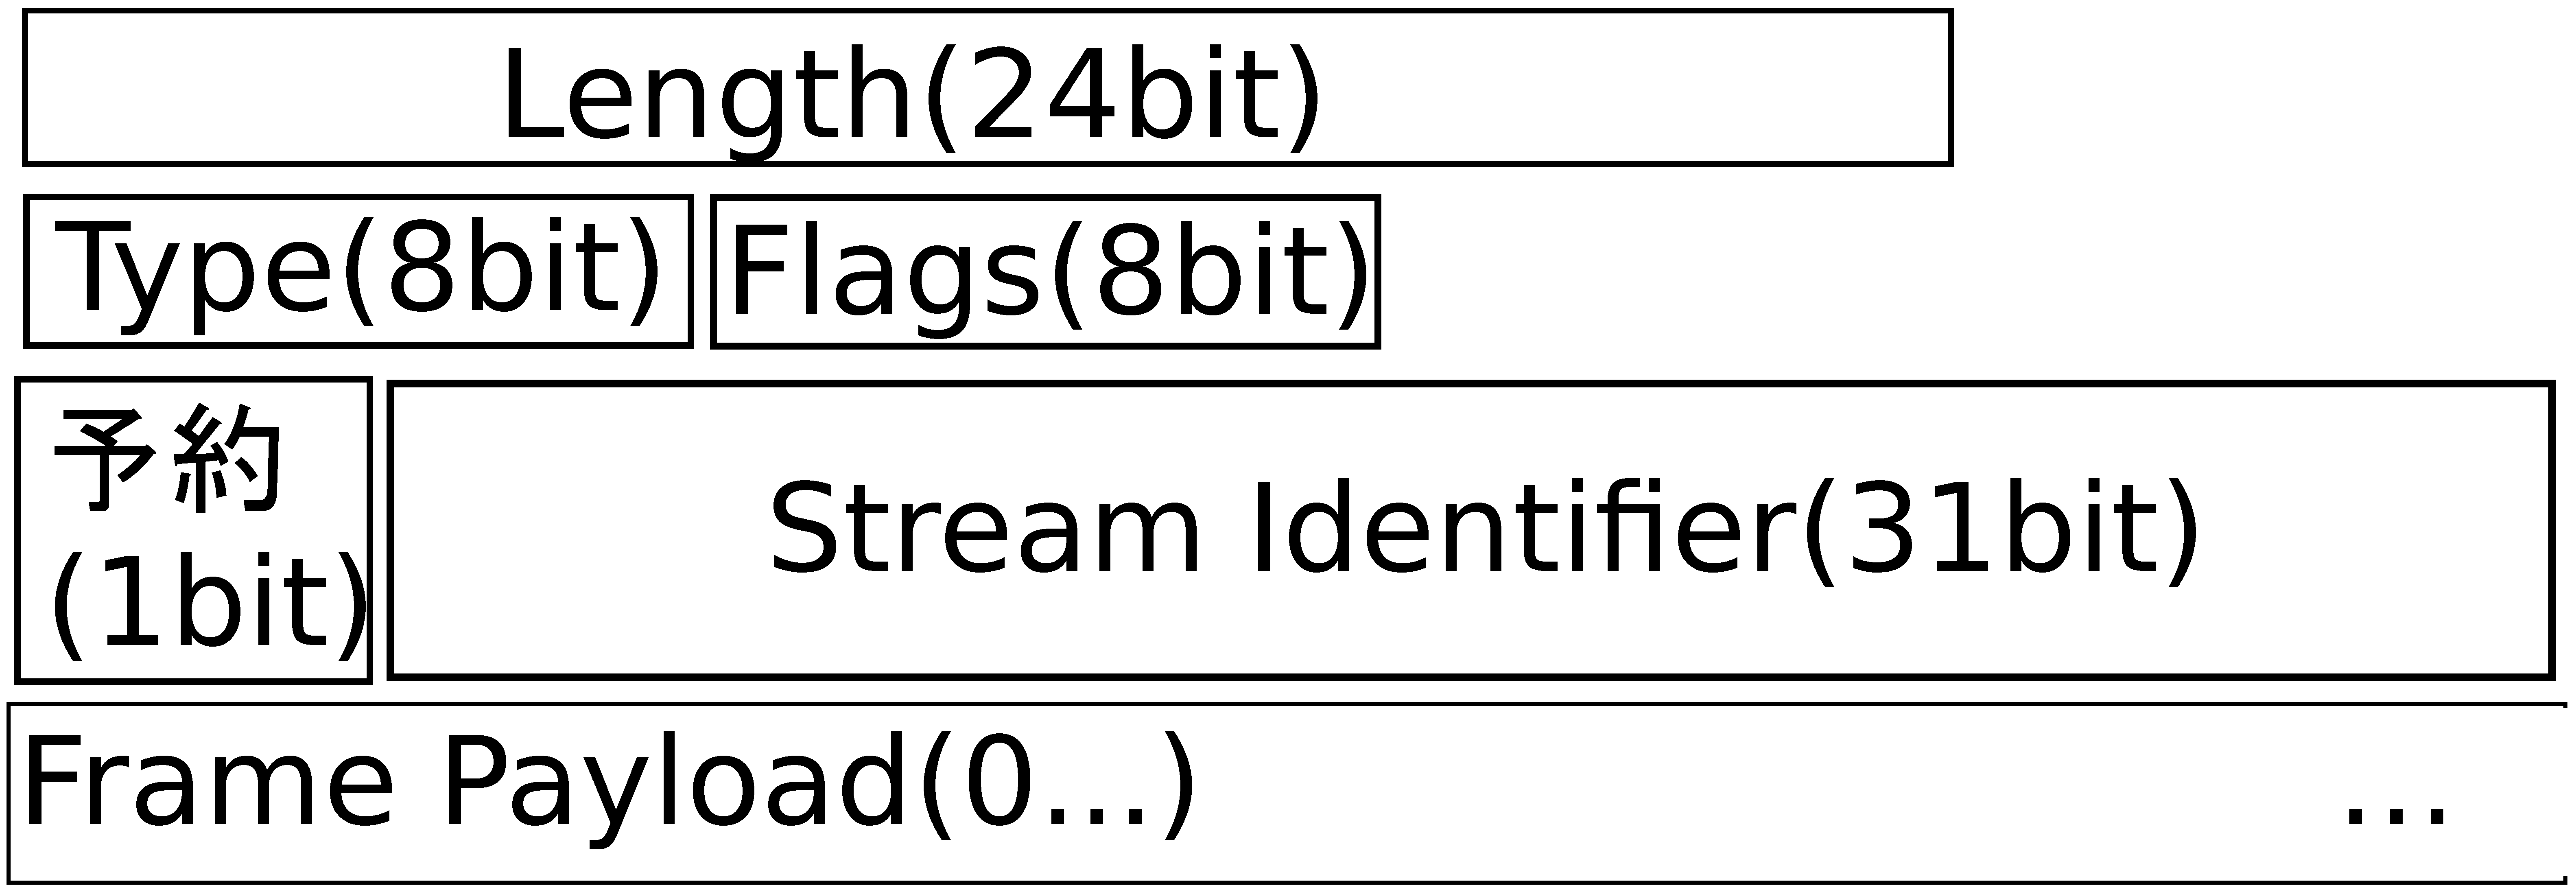
\includegraphics[width=80mm]{img/frame2.eps}
\caption{HTTP/2のフレーム}
\label{HTTP2frame}
\end{figure}

\begin{itemize}
 \item  Length:Frame Payloadの長さ
 \item Type:どんな通信メッセージか
 \item Flags:Typeによっては真偽フラグに使うため予約されている
 \item Stream Identifier:ストリームID
 \item Frame Payload:通信メッセージの内容
\end{itemize}

「フレーム」は今までのテキストではなく数値のみであり
バイナリ形式によって決まっており人間には理解しにくい.
\\ しかし,人間には理解しにくくなったがバイナリにしたことで
データ量が減り,形が決まっているので間違いが少なくなる.


\subsection{HTTPヘッダ圧縮}
HTTPの要求と応答には,「HTTPヘッダ」が含まれている.
HTTPヘッダはHTTPで通信するためのデータやどんな情報が送られてきたかなどの情報がある.
\\ しかし,HTTPヘッダの中にはブラウザの情報など同じHTTPヘッダが何度も送られている.
そのため無駄なデータのやり取りをしていることになる.
\\ HTTP/2ではHTTPヘッダを圧縮し無駄なデータのやり取りを減少させている.



\subsection{サーバから必要なデータの付与}
HTTP/2からはブラウザが要求をサーバに送り,
サーバがブラウザに応答を返すときに要求に関係のあるデータを送ることができる機能である.
\\ 例えば,Webページをの要求をブラウザが送ると
HTTP/1.1ではサーバはWebページの情報のみを返している.
\\ しかし,HTTP/2からはそのページで表示する画像も一緒に送ることができる.
\\ よって,HTTP/2では後からブラウザが要求を送らなくても
関係しているデータを先にもらうことができる.



\section{HTTP/2今後}
HTTP/2を使うためにはサーバとブラウザの両方が対応して初めて使うことができる.
\\ 主要ブラウザの最新バージョンはHTTP/2に対応しており「Windows10」の「Internet Explorer11」,「Firefox36」,「Google Chrome 40」などがある.
\\ Goolge ChromeやFirefoxではセキュリティのある
HTTP/2のみをサポートするなどセキュリティ面での向上も考えられる.
\\ HTTP/2はまだ完全な仕様が決定していないなど
まだまだこれから発展していくものであり恩恵を受けるためにはまだ時間がかかると考えられる.
\\ しかし,Googleやtwitterなどにはすでに導入がされており
これからさらに導入が加速されていくと思われる.




\small
\bibliographystyle{junsrt}
\bibliography{bib}
%------------------------------------------------------------------------------
\end{document}
